

\subsection{Vecindades}

Para poder observar cuantos pixeles vecinos deb\'iamos tomar en cuenta para encontrar la direcci\'on de la luz procedimos a hacer un breve experimento donde pintabamos de distintos colores los pixeles que consideraba mas brillante dependiendo la cantidad de vecindades. En este caso, donde mejor se pudo apreciar visualmente, se observa el punto negro con 0 vecindades (Solo \'el mismo), el punto rojo considera 2 pixeles vecinos, el punto verde son 4, el azul 6 vecindades, el amarillo 8 y el cian 10 pixeles vecinos.


\begin{center}
   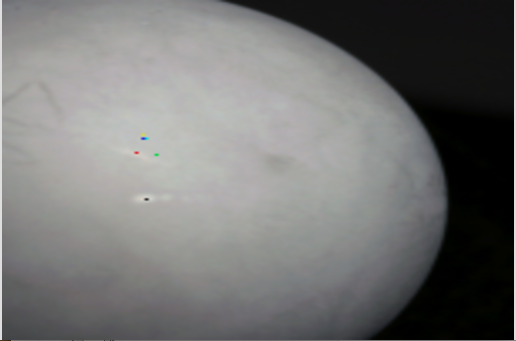
\includegraphics[scale=0.6]{ejemplo.png}
   \label{Fig. 1}
   \caption{Vecindades en esfera}
\end{center}

Prosiguiendo con las misma idea y utilizando las direcciones de luz obtenidas con vecindad 0 y vecindad 6,la cual consideramos la optima, obtuvimos distintos campos normales para la im\'agen del buda, observables a continuaci\'on:


\begin{center}
   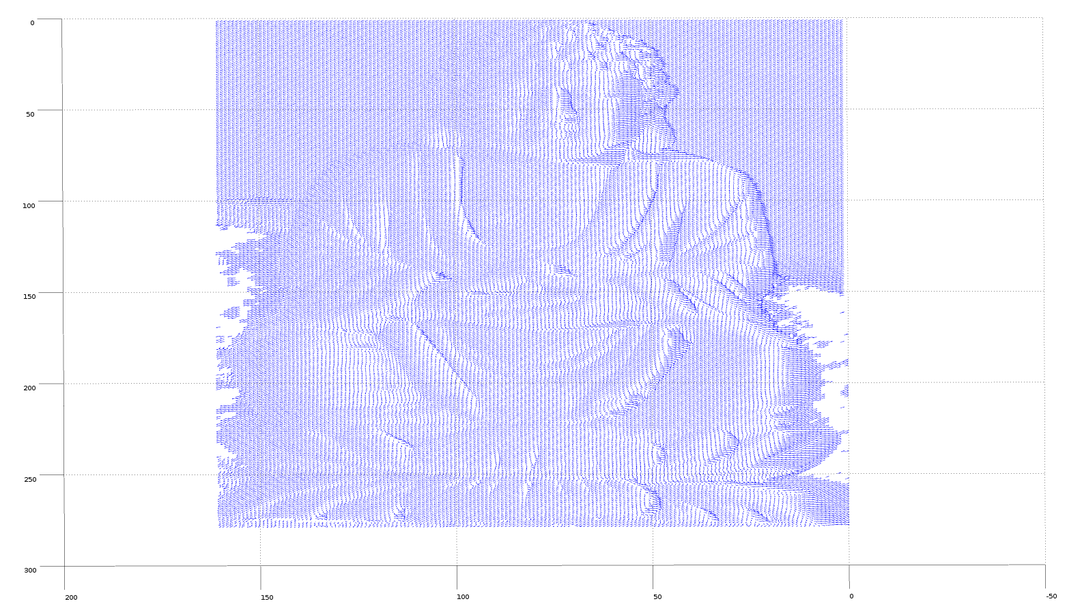
\includegraphics[scale=0.4]{buda_vecindad_0.png}
   \label{Fig. 2}
   \caption{Buda con vecindad 0}
\end{center}

\begin{center}
   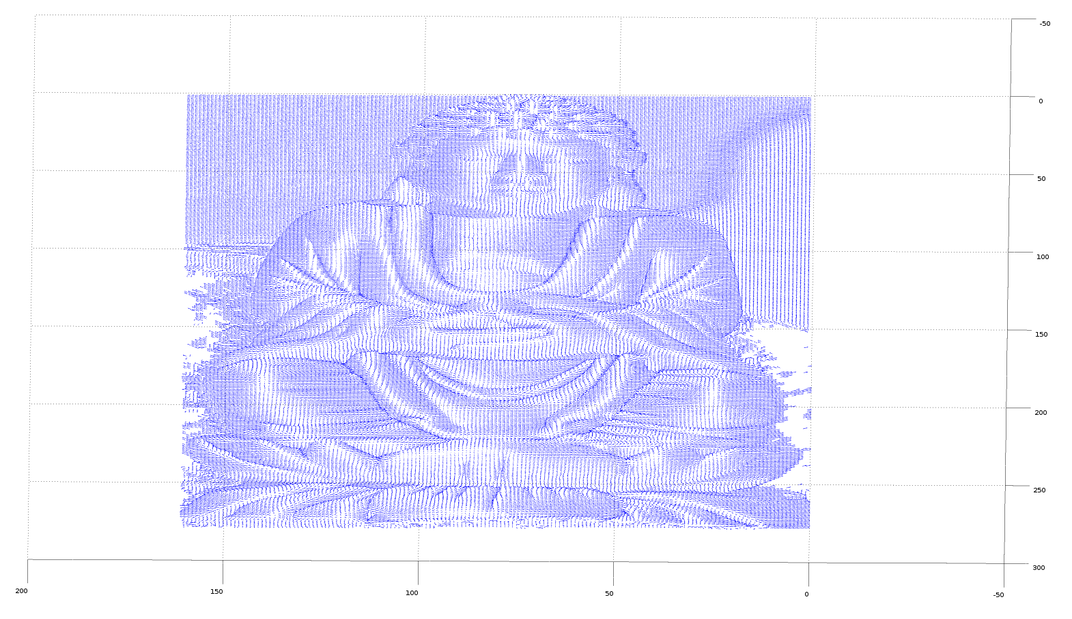
\includegraphics[scale=0.4]{buda_vecindades_6.png}
   \label{Fig. 3}
   \caption{Buda con vecindad 6}
\end{center}


\indent La im\'agen se observan esos factores de los que hablamos en el desarrollo, entre aquellos, las manchas de distinto color y la aureola de luz. P\'or ejemplo se ve el de vecindad 0 (p\'unto negro) bi\'en lejos de los demas, por lo claro de la mancha blanca. Las vecindades de 2 y 4 (rojo y verde) tambi\'en fueron corrompidos por el ruido, aunque llegaron un poco mas cerca. Luego a partir de los 6, 8 y 10 (az\'ul, amar\'illo y cian) se podria creer que llega a un lugar en donde por m\'as que agrandes el n\'umero de cantidad de vecindades no modificaria la posici\'on, tambi\'en vi\'endolo a simple vista se puede corroborar que es de d\'onde uno diria que proviene la luz.
Luego en el pr\'oximo experimento se observa que al modificar la cantidad de vecindades repercute fuertemente en la realizacion del resto del modelo, ya que con una mala direcci\'on de la luz se perdera el efecto 3D, o mas bien parecera como que se obtuvo el efecto solo de uno de los lados (de derecha a izquierda). \par



\subsection{N\'umero de condici\'on}

La mejor forma de ver la diferencia entre dos matrices con distintos n\'umeros de condici\'on fue tomar la matrices con menor y con mayor n\'umero de condici\'on asociados. De esta manera obtuvimos una matriz con un n\'umero de 15.0503 y otro con 407.581, una gran diferencia de tama�os. Luego para poder observar visualmente la dicerencia se le calculo el campo normal a cada uno, el resultado es el siguiente:



\begin{center}
   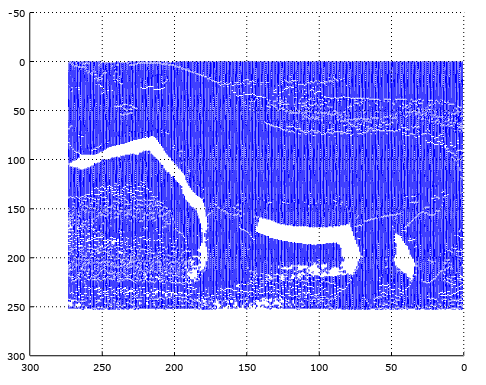
\includegraphics[scale=0.6]{caballoMax.png}
   \label{Fig. 4}
   \caption{Caballo con N\'umero de condici\'on de 407.581}
\end{center}

\begin{center}
   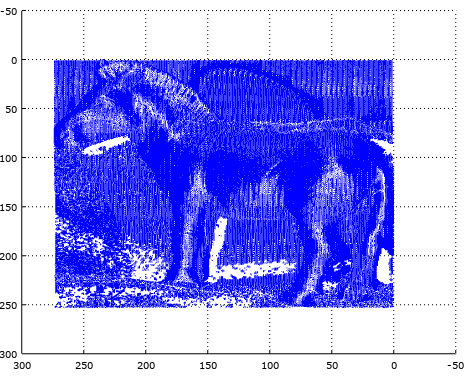
\includegraphics[scale=0.6]{caballoMin.png}
   \label{Fig. 5}
   \caption{Caballo con N\'umero de condici\'on de 15.0503}
\end{center}


\subsection{Complejidades algoritmicas}

*********************

\indent Nuestra primer idea para tratar de comprobar nuestra hip�tesis de que la factorizaci\'on LU es mas r\'apida que la eliminaci\'on de gauss fue tomar distintos tama�os de matrices y triangularlos una vez con cada algoritmo para ver que m�todo era mas r\'apido. Este experimento no pone a prueba nuestra hip\'otesis porque lo que intent\'abamos comprobar es que la factorizaci\'on LU es mas r\'apida que la eliminaci\'on de gauss para resolver un sistema lineal despues de la primera vez que se resuelve el sistema. Si resolv\'iamos una sola vez cada tama�o de matriz, ambos algoritmos tardar\'ian lo mismo. Por lo tanto, decidimos hacer un experimento donde mantuvimos constante el tama�o del sistema lineal a resolver y lo que variamos en cada instancia de testeo fueron las cantidades de t\'erminos independientes que debia resolver. Agregamos al mismo experimento la factorizaci\'on de Cholesky.

\begin{center}
   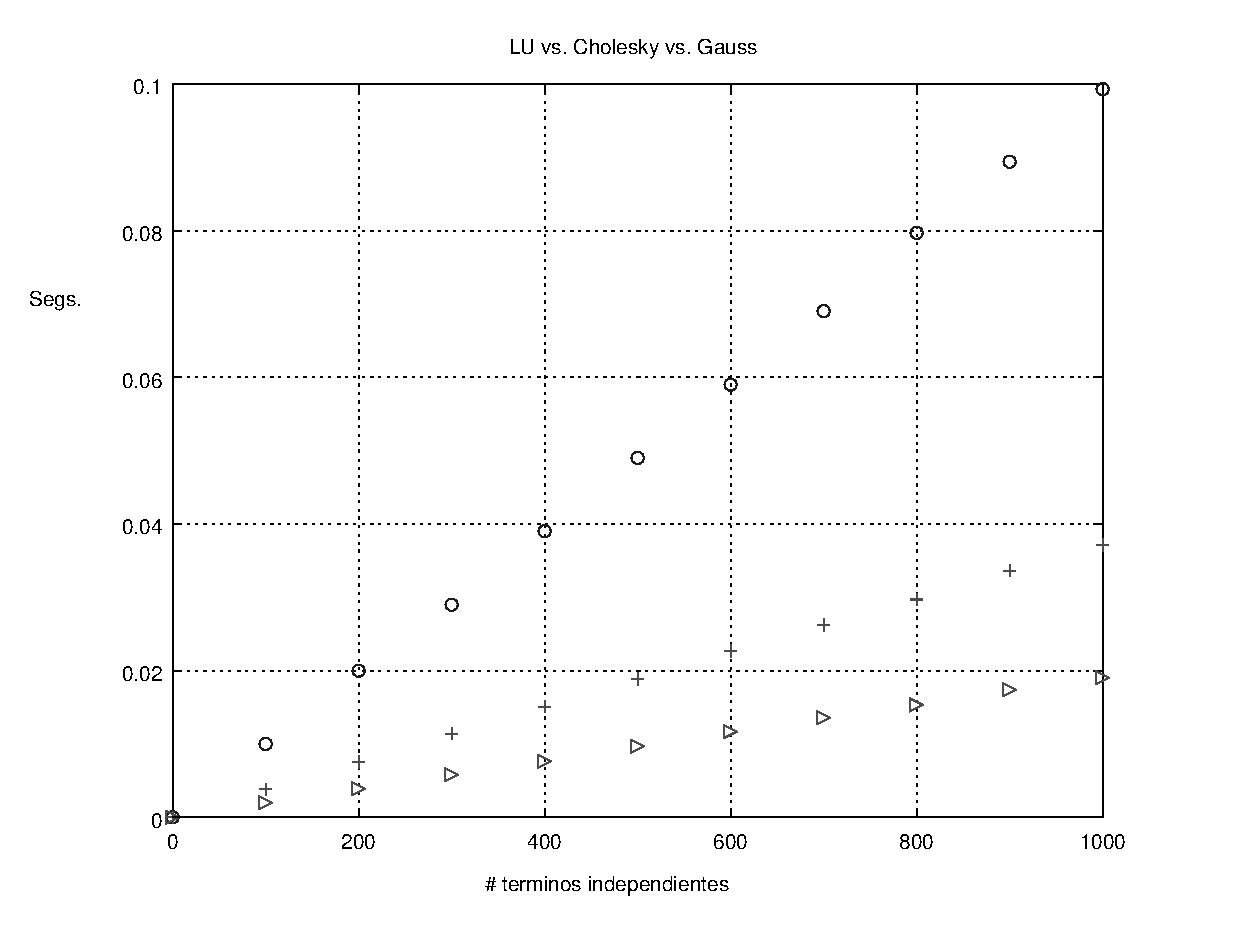
\includegraphics[scale=0.6]{LuCholeGauss.eps}
   \label{Fig. 6}
   \caption{Resultado obtenido al aumentar la cantidad de terminos independientes}
\end{center}

\indent Nuestra hipotes\'i�s, y a partir de lo que nos comentaron en las clases era que los algoritmos de eliminaci\'on gaussiana, factorizaci\'on LU y Cholesky iban a tener un orden de complejidad c\'ubico y cuadrado, respectivamente, lo que al ver los resultados de las experimentaciones nos dice lo contrario. Las complejidades nos resultaron lineales.
Luego de consultarlo con la catedra, pudimos comprender que las complejidades no se iban a ver reflejadas en este experimento, ya que el tama�o de la matriz se mantenia igual. Por lo tanto debimos realizar un nuevo experimento en donde dejamos fijos en 100 terminos independientes a resolver y lo que se variaba en cada corrida era el tama�o de las matrices.

*** Foto nueva ***